%\section{Waveform Interface}

This chapter explains some of the features of the waveform interface. The interface is defined in a flexible way to accommodate a diverse set of waveforms. 

\section{Overview}

The waveform interface serves as the lower interface of the Tuscarora Framework.  Any waveform that satisfies the interface definition may be plugged into the Framework for use alongside other waveforms, in order to support a heterogeneous MANET.

To satisfy the waveform interface, a waveform provider needs to implement a single interface, called \CPPClassName{Waveform\_I}.  The interface, \CPPClassName{Waveform\_I} is a template class that is instantiated by passing the waveform’s address type as a template parameter.  In total, there are 10 methods in each instantiated class, of which 3 are optional, that is, a waveform provider can choose to not implement any or all of the optional methods. \cref{Fig:WaveformModules} shows the waveform
interfaces as related to the framework interfaces.


\begin{figure}[h]
 \centering
 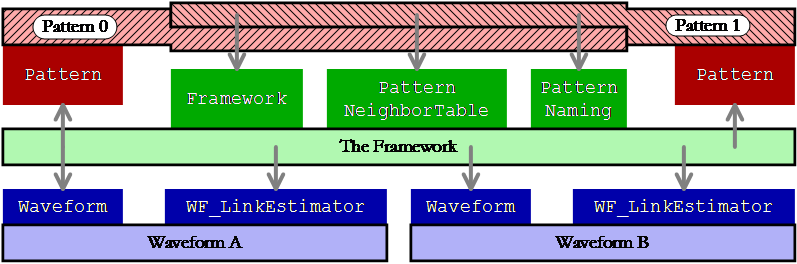
\includegraphics[width=0.9\linewidth]{figures/WaveformModules}
 \caption{Waveform Interfaces}
 \label{Fig:WaveformModules}
\end{figure}

Please refer to the Framework API documentation for full detail about the \CPPClassName{Waveform\_I} interface. 


\subsection {Programming Style:  Syntax and Semantics}
The interface design uses asynchronous message passing semantics, with a functional syntax, to define interactions between the waveform and Tuscarora.  It consists of two sorts of methods:  1) incoming commands, exercised by the user of the interface (namely, the Framework, via a communication shim) on the waveform, and 2) outgoing events, sent by the waveform to the user of the interface.

In terms of syntax, both commands and events are specified using function calls.  This simple representation yields ease of programming and, equally importantly, avoids restriction to a particular implementation of method invocation, such as socket communications between processes, which may be appropriate for some use cases (e.g., on large hardware platforms) but not others (e.g., for ns-3 simulation platforms where the overhead seems to matter).

In terms of semantics, all interface methods are explicitly associated with a message passing semantics.  The message passing semantics is reflected by the fact that all incoming commands have a return type of void.  Moreover, for any command that expects some sort of response from the waveform, an associated event method exists in the waveform interface, to convey the result of the computation.

The design assumes that a communication library, which we colloquially refer to as a “shim-layer”, is provided that implements the invocation of command and event methods using asynchronous message  passing.  The slightly different shim layer might be required for each waveform-platform pair, although generally far fewer shim layers would be required.

\subsection {Data Plane and Control Plane}
The waveform interface functionality spans a Data Plane and a Control Plane.  The Data Plan interface consists of the functions SendData, BroadcastData, Data Notification Event and the Received Message Event.  The remaining commands and events, as detailed below, which deal with the control status of the waveform, link estimation and schedules comprise the Control Plane. Figure 1 shows the Summary of the Commands and the Events that are expected by the framework in response to them, split across the Data and Control planes. The dotted lines show the dependency between a command and the event. 

\subsection {Interface Interaction Pattern using Asynchronous Message Passing}
In general, the data and control plane functions follow a common interaction pattern.  A command originates from Tuscarora to the waveform and, subsequently, one or more corresponding events are sent from the waveform back to the Framework.  Events are mapped and routed to particular modules and/or function within the Framework; it is convenient to think of each event as “named pipe” between the waveform and the Framework.  Each event is specified as a class with a single “Invoke” method that has a specific type of parameter. The Invoke method returns a bool (as against the void return type of most commands). The return type of Invoke indicates the status of queuing the Event on to the communication mechanism. The return type does not indicate the success or failure of sending the event to the framework. For example, if an Invoke returned a ‘true’ it means that the shim layer responsible for the communication has accepted the event and has queued it up for sending at a latter time. If it returns a ‘false’, it means either the communication mechanism is either broken or is busy processing existing events and cannot accept any new events to be sent out.
Five types of events are defined for the waveform:
\begin{enumerate}
\item Received Message Event (WF\_RcvMessageEvent\_t):  This Event is sent whenever a data message is received on the waveform, with WF\_RecvMsgParam  as the parameter.
\item	Data Notification Event (WF\_DataNotifierEvent\_t):  This Event is sent to convey the status of the SendData and BroadcastData calls and the WF\_DataNotifierParam is used as the event parameter. This Event might be generated up to three times for each data message, once to acknowledge the message has been received by the waveform, once when it is sent out and once when the message is received at the destination.
\item	Control Response Event (WF\_ControlResponseEvent\_t):  This Event is sent in response to one of the request commands in the control plane with WF\_ControlRssponseParam as the parameter. The parameter contains a response type, response status (success/failure), any additional data and its size.
\item	Link Estimation Event (WF\_LinkEstimateEvent\_t):  This Event is sent to provide to the Framework link estimates updates about a neighbor. The WF\_LinkEventParam is used as the parameter for this event.
\item	Schedule Update Event (WF\_ScheduleUpdateEvent\_t):  This Event is sent by the waveform to provide updates about its sending or receiving schedules. WF\_ScheduleUpdateParam is used as the event parameter.
\end{enumerate}

Every command originating from the Framework has a sequence number and the events use the same sequence number to identify their response.  The Framework tracks the sequence number it uses for each command and if it fails to receive a response for some command, it may resend that command with the same sequence number.  The waveform using the same sequence number to send multiple response to the same command or to update/change the response to the command is acceptable.  For the control plane commands the sequence number is called as the “RequestId”, for the data plane it is called as the “MessageId”.  A couple of special cases are allowed:  The Link Estimation Event and the Schedule Update Event do not use sequence numbers in their events and error recovery is not provided for those events.  For the Received Message Event the sequence number is generated by the Waveform and sent to the Framework.

\subsection {Control Plane State}

As far as the Framework’s awareness of the control state of the waveform is concerned, it knows only that the state of the waveform can be one of the following states which are defined by the enum WF\_ControlP\_StatusE:
\begin{itemize}
	\item WF\_NORMAL:  Waveform has been initialized and is operating within “normal” bounds.
	\item WF\_BUSY:  Waveform has been initialized, but is busy with non-data plane functions. The Framework should desist from sending messages to waveform, it is likely that the waveform might not accept the messages.
	\item WF\_ERROR:  Waveform is in an error state. The Framework should not send messages to waveform, until the status changes.
	\item WF\_BUFFER\_LOW:  The waveform is operating normally, but is at risk of running out of messages to send out. The Framework may respond by attempting to increase the data output to the waveform.
	\item WF\_BUFFER\_FULL:  The waveform is operating normally, but is at risk of being overrun by data packets. The Framework should respond by slow down its rate of invoking data packet sends on the waveform.
\end{itemize}


\subsection {Flow Control}
The Waveform accomplishes flow control between the Waveform and Framework in one of three ways:

\begin{enumerate}
	\item	Waveform can drop the packet being sent to it and return a negative status when sending a data notification message back to the Framework.  The Framework will interpret this as the waveform not being ready to receive data messages.
	\item	Waveform can send a WF\_BUFFER\_LOW or WF\_BUFFER\_FULL response messages to the Framework, to request it to speed up or slow down the data message rate.
	\item	Waveform can send a WF\_ERROR status message to completely stop receiving any data messages from the Framework if it has to clear a backlog.  It could subsequently send a WF\_NORMAL status message when it is ready to resume.
	The remaining sections describe the API methods (first commands, then events) in detail.
\end{enumerate}

\subsection {Parameter Ownership}
In Tuscarora whenever a function call happens across layers the ownership of the data structures passed as parameters is transferred to the callee. In this particular case, this applies to the commands the Waveform\_I interface receives and the event calls the waveform makes. We call the “Give” model of ownership where the ownership is given when to the callee. The Give model is used to avoid deep copying of packets and other parameters at the callee so that efficiency of processing can be improved. However, there are some implications of this “Give” model. 
\begin{itemize}
\item Pass by reference: Any large parameter objects should be passed by reference in a function to make optimum use of the Give model. Passing by value does not utilize the Give model. However, for small objects this might not matter much.

\item Allocation on heap: The caller must also be explicitly aware of which parameters are passed as references, since these objects must be allocated on the heap (and not on the local stack). Creating a local object and passing this as reference to another method will result in run time errors. Also, once a parameter has been passed as reference and the call has been made, the same object cannot be modified by the caller anymore. This would also result in run time errors.

\item Deallocation:  It is the callee’s responsibility to deallocate any parameter that is  passed by reference, since these were originally allocated on the heap by the caller. Failing to deallocate (or reuse) such objects will result in a memory leak. 
\end{itemize}



\section{Packet Metadata}

Waveforms should also provide metadata for each packet received.
The metadata provided is standardized across all
waveforms. Currently 3 types of metadata have been defined, (i)
Received signal strength indicator (RSSI), (ii) Signal to noise and
interference ratio (SINR) and (iii) Packet reception time stamp.
The metadata is used by the framework to create and/or improve the
estimates for the properties of links.
%estimates of the the neighbors.

\if false
\begin{lstlisting}[style=boralargefile][captionpos=b,caption={Waveform attributes structure used to expose information about the waveform to framework},label=List:Attributes]
 
struct WaveformAttributes{
  uint16_t wfId;		///Waveform Ids given by the framework
  WF_TypeE type;		///Type of waveform	
  WF_EstimatorTypeE estType;	///Type of estimator provided by the waveform
  WF_AntennaTypeE antType;	///Type of antenna used by the waveform
  WF_ModeE mode;		///Current mode of the waveform
  uint16_t ifindex;		///Waveform OS/Platform interfce index number
  char name[32];		///Name of waveform
  uint16_t headerSize;		///Size of the waveform header in bytes
  uint16_t maxPayloadSize;	///Maximum payload that can be sent on the waveform in 			bytes
  uint16_t maxPacketSize;	///Maximum packet size that can be sent on the waveform 			(in bytes), including the waveform header
  uint16_t minPacketSize;	///Minimum packet size that can be sent on the waveform 			(in bytes), including the waveform header
  uint32_t minInterPacketDelay; ///Minimum interpacket rate in micro seconds
  uint32_t channelRate; 	///The channel rate in bytes per second
  uint32_t maxBurstRate; 	///Maximum data burst rate in bytes per second
};
\end{lstlisting}

\fi

%\hypertarget{class_waveform_1_1_waveform_base}{}\section{Waveform\+:\+:Waveform\+Base Class Reference}
\label{class_waveform_1_1_waveform_base}\index{Waveform\+::\+Waveform\+Base@{Waveform\+::\+Waveform\+Base}}


Inheritance diagram for Waveform\+:\+:Waveform\+Base\+:\nopagebreak
\begin{figure}[H]
\begin{center}
\leavevmode
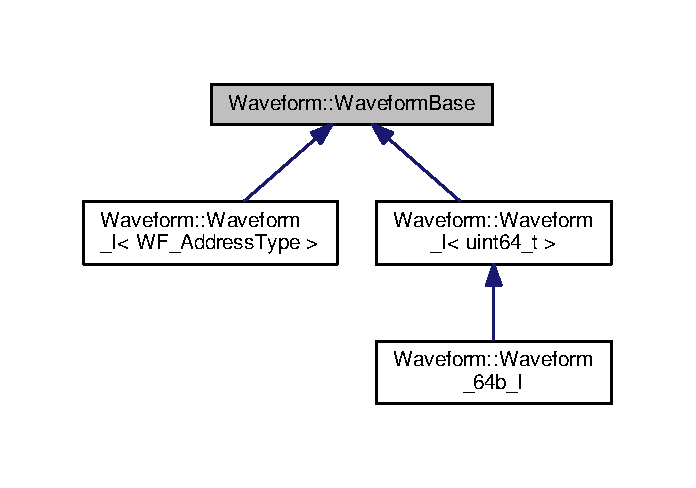
\includegraphics[width=334pt]{class_waveform_1_1_waveform_base__inherit__graph}
\end{center}
\end{figure}
\subsection*{Public Member Functions}
\begin{DoxyCompactItemize}
\item 
virtual void \hyperlink{class_waveform_1_1_waveform_base_a67053c3a29b7fa3f477dce71a15fc624}{Replace\+Payload\+Request} (Request\+Id\+\_\+t r\+Id, W\+F\+\_\+\+Message\+Id\+\_\+t msg\+Id, uint8\+\_\+t $\ast$payload, uint16\+\_\+t payload\+Size)=0
\begin{DoxyCompactList}\small\item\em Requests the replacement the payload of a message, passed in an earlier call to ‘\+Send\+Data’ or ‘\+Broadcast\+Data’ method with the given Message\+Id. The previous payload will be discarded. \end{DoxyCompactList}\item 
virtual void \hyperlink{class_waveform_1_1_waveform_base_aad9cfbc04a5168caa1780edd812d6f7d}{Attributes\+Request} (Request\+Id\+\_\+t r\+Id)=0
\begin{DoxyCompactList}\small\item\em Request the attributes of the waveform. \end{DoxyCompactList}\item 
virtual void \hyperlink{class_waveform_1_1_waveform_base_ac5a64312ea70923af969c51cc4e0363d}{Control\+Status\+Request} (Request\+Id\+\_\+t r\+Id)=0
\begin{DoxyCompactList}\small\item\em Requests the control status of waveform. A W\+F\+\_\+\+StatusE enum type is sent as the data of the response message, to indicate the status of the variable. \end{DoxyCompactList}\item 
virtual void \hyperlink{class_waveform_1_1_waveform_base_a767db0e1d92d0e3ae46da3b2335e9b87}{Data\+Status\+Request} (Request\+Id\+\_\+t r\+Id, W\+F\+\_\+\+Message\+Id\+\_\+t m\+Id)=0
\begin{DoxyCompactList}\small\item\em Requests the status of a data message already sent to the waveform. \end{DoxyCompactList}\item 
virtual void \hyperlink{class_waveform_1_1_waveform_base_ad0e6f375f176315332c7e90d57fb8a21}{Set\+Schedule\+Request} (Request\+Id\+\_\+t r\+Id, Node\+Id\+\_\+t node\+Id, W\+F\+\_\+\+Schedule\+TypeE type, Schedule\+BaseI \&schedule, uint16\+\_\+t schedule\+Size)
\begin{DoxyCompactList}\small\item\em Sends information about a schedule for one of 3 kinds of functions\+: link estmation, sending or receiving to the waveform. \end{DoxyCompactList}\item 
virtual void {\bfseries Schedule\+Request} (Request\+Id\+\_\+t r\+Id, Node\+Id\+\_\+t nodeid, W\+F\+\_\+\+Schedule\+TypeE type)\hypertarget{class_waveform_1_1_waveform_base_ac443d02d12315ac2aeb4cb0f62c35862}{}\label{class_waveform_1_1_waveform_base_ac443d02d12315ac2aeb4cb0f62c35862}

\end{DoxyCompactItemize}


\subsection{Member Function Documentation}
\index{Waveform\+::\+Waveform\+Base@{Waveform\+::\+Waveform\+Base}!Attributes\+Request@{Attributes\+Request}}
\index{Attributes\+Request@{Attributes\+Request}!Waveform\+::\+Waveform\+Base@{Waveform\+::\+Waveform\+Base}}
\subsubsection[{\texorpdfstring{Attributes\+Request(\+Request\+Id\+\_\+t r\+Id)=0}{AttributesRequest(RequestId_t rId)=0}}]{\setlength{\rightskip}{0pt plus 5cm}virtual void Waveform\+::\+Waveform\+Base\+::\+Attributes\+Request (
\begin{DoxyParamCaption}
\item[{Request\+Id\+\_\+t}]{r\+Id}
\end{DoxyParamCaption}
)\hspace{0.3cm}{\ttfamily [pure virtual]}}\hypertarget{class_waveform_1_1_waveform_base_aad9cfbc04a5168caa1780edd812d6f7d}{}\label{class_waveform_1_1_waveform_base_aad9cfbc04a5168caa1780edd812d6f7d}


Request the attributes of the waveform. 

{\bfseries Semantic Behavior\+:} \hyperlink{namespace_waveform}{Waveform} should return its attributes to the Framework by generating a response through the Control Response Event, with the same request ID. The status of the response message should be true, unless otherwise the attributes are not available to be sent to the Framework. The response contains attributes in the \hyperlink{struct_waveform_1_1_w_f___attributes}{W\+F\+\_\+\+Attributes} structure, which is copied into the data portion of the \hyperlink{struct_waveform_1_1_w_f___control_response_param}{W\+F\+\_\+\+Control\+Response\+Param}.


\begin{DoxyParams}{Parameters}
{\em r\+Id} & Specifies the ID of the request, which the waveform will use to in its response message. \\
\hline
\end{DoxyParams}
\begin{DoxyReturn}{Returns}
void. 
\end{DoxyReturn}


Implemented in \hyperlink{class_waveform_1_1_waveform__64b___i_a11e3bb3d2db8b8f1f7f63159782af9ce}{Waveform\+::\+Waveform\+\_\+64b\+\_\+I}.

\index{Waveform\+::\+Waveform\+Base@{Waveform\+::\+Waveform\+Base}!Control\+Status\+Request@{Control\+Status\+Request}}
\index{Control\+Status\+Request@{Control\+Status\+Request}!Waveform\+::\+Waveform\+Base@{Waveform\+::\+Waveform\+Base}}
\subsubsection[{\texorpdfstring{Control\+Status\+Request(\+Request\+Id\+\_\+t r\+Id)=0}{ControlStatusRequest(RequestId_t rId)=0}}]{\setlength{\rightskip}{0pt plus 5cm}virtual void Waveform\+::\+Waveform\+Base\+::\+Control\+Status\+Request (
\begin{DoxyParamCaption}
\item[{Request\+Id\+\_\+t}]{r\+Id}
\end{DoxyParamCaption}
)\hspace{0.3cm}{\ttfamily [pure virtual]}}\hypertarget{class_waveform_1_1_waveform_base_ac5a64312ea70923af969c51cc4e0363d}{}\label{class_waveform_1_1_waveform_base_ac5a64312ea70923af969c51cc4e0363d}


Requests the control status of waveform. A W\+F\+\_\+\+StatusE enum type is sent as the data of the response message, to indicate the status of the variable. 

{\bfseries Semantic Behavior\+:} The Framework expects the waveform to be in one of the data plane states defined by the W\+F\+\_\+\+Control\+P\+\_\+\+StatusE enum. The waveform should return the current status of its data plane by generating a response through the Control Response Event, with the same Request\+Id. The status that response message should be true. The actual data plane status should be copied into the data part of the response


\begin{DoxyParams}{Parameters}
{\em r\+Id} & Specifies the ID of the request, which the waveform will use to in its response message. \\
\hline
\end{DoxyParams}
\begin{DoxyReturn}{Returns}
void. 
\end{DoxyReturn}


Implemented in \hyperlink{class_waveform_1_1_waveform__64b___i_ae13e7e49359ea2e45b010cdf4f1d3227}{Waveform\+::\+Waveform\+\_\+64b\+\_\+I}.

\index{Waveform\+::\+Waveform\+Base@{Waveform\+::\+Waveform\+Base}!Data\+Status\+Request@{Data\+Status\+Request}}
\index{Data\+Status\+Request@{Data\+Status\+Request}!Waveform\+::\+Waveform\+Base@{Waveform\+::\+Waveform\+Base}}
\subsubsection[{\texorpdfstring{Data\+Status\+Request(\+Request\+Id\+\_\+t r\+Id, W\+F\+\_\+\+Message\+Id\+\_\+t m\+Id)=0}{DataStatusRequest(RequestId_t rId, WF_MessageId_t mId)=0}}]{\setlength{\rightskip}{0pt plus 5cm}virtual void Waveform\+::\+Waveform\+Base\+::\+Data\+Status\+Request (
\begin{DoxyParamCaption}
\item[{Request\+Id\+\_\+t}]{r\+Id, }
\item[{W\+F\+\_\+\+Message\+Id\+\_\+t}]{m\+Id}
\end{DoxyParamCaption}
)\hspace{0.3cm}{\ttfamily [pure virtual]}}\hypertarget{class_waveform_1_1_waveform_base_a767db0e1d92d0e3ae46da3b2335e9b87}{}\label{class_waveform_1_1_waveform_base_a767db0e1d92d0e3ae46da3b2335e9b87}


Requests the status of a data message already sent to the waveform. 

{\bfseries Semantic Behavior\+:} If the Framework is uncertain about the status of a message that it sent to the waveform, it can send the Data\+Status\+Request command. A response message should be generated through the Control Response Event, with the same Request\+Id, that should have the status set as ‘true’ if the waveform received the particular message and a W\+F\+\_\+\+Data\+Notifier\+Param object must be created that reflects the current status of the message and should be copied into the data part of the \hyperlink{struct_waveform_1_1_w_f___control_response_param}{W\+F\+\_\+\+Control\+Response\+Param}.


\begin{DoxyParams}{Parameters}
{\em r\+Id} & Specifies the ID of the request, which the waveform will use to in its response message. \\
\hline
{\em m\+Id} & Specified the ID of the message, for which status is requested. \\
\hline
\end{DoxyParams}
\begin{DoxyReturn}{Returns}
void. 
\end{DoxyReturn}


Implemented in \hyperlink{class_waveform_1_1_waveform__64b___i_a06bcaf416cc353850232ee373b3bac01}{Waveform\+::\+Waveform\+\_\+64b\+\_\+I}.

\index{Waveform\+::\+Waveform\+Base@{Waveform\+::\+Waveform\+Base}!Replace\+Payload\+Request@{Replace\+Payload\+Request}}
\index{Replace\+Payload\+Request@{Replace\+Payload\+Request}!Waveform\+::\+Waveform\+Base@{Waveform\+::\+Waveform\+Base}}
\subsubsection[{\texorpdfstring{Replace\+Payload\+Request(\+Request\+Id\+\_\+t r\+Id, W\+F\+\_\+\+Message\+Id\+\_\+t msg\+Id, uint8\+\_\+t $\ast$payload, uint16\+\_\+t payload\+Size)=0}{ReplacePayloadRequest(RequestId_t rId, WF_MessageId_t msgId, uint8_t *payload, uint16_t payloadSize)=0}}]{\setlength{\rightskip}{0pt plus 5cm}virtual void Waveform\+::\+Waveform\+Base\+::\+Replace\+Payload\+Request (
\begin{DoxyParamCaption}
\item[{Request\+Id\+\_\+t}]{r\+Id, }
\item[{W\+F\+\_\+\+Message\+Id\+\_\+t}]{msg\+Id, }
\item[{uint8\+\_\+t $\ast$}]{payload, }
\item[{uint16\+\_\+t}]{payload\+Size}
\end{DoxyParamCaption}
)\hspace{0.3cm}{\ttfamily [pure virtual]}}\hypertarget{class_waveform_1_1_waveform_base_a67053c3a29b7fa3f477dce71a15fc624}{}\label{class_waveform_1_1_waveform_base_a67053c3a29b7fa3f477dce71a15fc624}


Requests the replacement the payload of a message, passed in an earlier call to ‘\+Send\+Data’ or ‘\+Broadcast\+Data’ method with the given Message\+Id. The previous payload will be discarded. 

{\bfseries Semantic Behavior\+:} \hyperlink{namespace_waveform}{Waveform} should replace the payload of a message passed in an earlier call to ‘\+Send\+Data’ or ‘\+Broadcast\+Data’ method with the given message ID, if the message has not been sent out. A response message should be generated through the Control Response Event, with the same request ID, that should include a status which will be set to false if the message has been sent out or if the waveform is unable to replace the payload of a message. Otherwise, the status should be set to true in the response message.


\begin{DoxyParams}{Parameters}
{\em r\+Id} & Specifies the ID of the request, which the waveform will use to in its response message. \\
\hline
{\em msg\+Id} & specifies the message ID of the packet. \\
\hline
{\em payload} & pointer to the new payload. \\
\hline
{\em payload\+Size} & size of the new payload. \\
\hline
\end{DoxyParams}
\begin{DoxyReturn}{Returns}
void. 
\end{DoxyReturn}


Implemented in \hyperlink{class_waveform_1_1_waveform__64b___i_a90bdc9d75233d1453c486ad200126b90}{Waveform\+::\+Waveform\+\_\+64b\+\_\+I}.

\index{Waveform\+::\+Waveform\+Base@{Waveform\+::\+Waveform\+Base}!Set\+Schedule\+Request@{Set\+Schedule\+Request}}
\index{Set\+Schedule\+Request@{Set\+Schedule\+Request}!Waveform\+::\+Waveform\+Base@{Waveform\+::\+Waveform\+Base}}
\subsubsection[{\texorpdfstring{Set\+Schedule\+Request(\+Request\+Id\+\_\+t r\+Id, Node\+Id\+\_\+t node\+Id, W\+F\+\_\+\+Schedule\+Type\+E type, Schedule\+Base\+I \&schedule, uint16\+\_\+t schedule\+Size)}{SetScheduleRequest(RequestId_t rId, NodeId_t nodeId, WF_ScheduleTypeE type, ScheduleBaseI &schedule, uint16_t scheduleSize)}}]{\setlength{\rightskip}{0pt plus 5cm}virtual void Waveform\+::\+Waveform\+Base\+::\+Set\+Schedule\+Request (
\begin{DoxyParamCaption}
\item[{Request\+Id\+\_\+t}]{r\+Id, }
\item[{Node\+Id\+\_\+t}]{node\+Id, }
\item[{W\+F\+\_\+\+Schedule\+TypeE}]{type, }
\item[{Schedule\+BaseI \&}]{schedule, }
\item[{uint16\+\_\+t}]{schedule\+Size}
\end{DoxyParamCaption}
)\hspace{0.3cm}{\ttfamily [inline]}, {\ttfamily [virtual]}}\hypertarget{class_waveform_1_1_waveform_base_ad0e6f375f176315332c7e90d57fb8a21}{}\label{class_waveform_1_1_waveform_base_ad0e6f375f176315332c7e90d57fb8a21}


Sends information about a schedule for one of 3 kinds of functions\+: link estmation, sending or receiving to the waveform. 

{\bfseries Semantic Behavior\+:} This method enables the Framework to pass on some scheduling information to the waveform. The expectation is that this method will be implemented only if the waveform needs scheduling information from the Framework or an external third party provider. The method enables receiving scheduling information specific to a neighbor specified by the \+\_\+node\+Id parameter. The schedule information is sent as abstract schedule object represented by the \+\_\+schedule object and the size of this object is specified by the \+\_\+schedule\+Size parameter. The expectation is that, if a waveform needs scheduling information, it will derive from the Schedule\+BaseI class and will implement its own scheduling class. The Framework defines three types of waveform schedules as the W\+F\+\_\+\+Schedule\+TypeE enum (one each for link estimation, sending, and receiving messages).

The waveform should regenerate a response to this request through the Control Response Event, with the same Request\+Id. The status of that response message should be true if the waveform able to successfully use the scheduler information or false otherwise.

Since this is an optional feature for waveforms, if it choose to implement it, the waveform should set the scheduler\+Info\+Support field in its Attribute as true whenever it responds to the Attribute\+Request.


\begin{DoxyParams}{Parameters}
{\em r\+Id} & Specifies the ID of the request, which the waveform will use to in its response message. \\
\hline
{\em nodeid} & Specifies the node ID for which the schedule should be used. \\
\hline
{\em type} & Enum that specifies the type of the schedule. There are 3 types of schedules, sending, receiving and link estimation. \\
\hline
{\em schedule} & Reference to an abstract schedule object. It is expected that this class will be derived and implemented by different waveforms. \\
\hline
{\em schedule\+Size} & Size of the schedule object. \\
\hline
\end{DoxyParams}
\begin{DoxyReturn}{Returns}
void. 
\end{DoxyReturn}


The documentation for this class was generated from the following file\+:\begin{DoxyCompactItemize}
\item 
Tuscarora\+F\+W/\+Include/\+Interfaces/\+Waveform/W\+F\+\_\+\+I.\+h\end{DoxyCompactItemize}



%\hypertarget{class_waveform_1_1_waveform___i}{}\section{Waveform\+:\+:Waveform\+\_\+I$<$ W\+F\+\_\+\+Address\+Type $>$ Class Template Reference}
\label{class_waveform_1_1_waveform___i}\index{Waveform\+::\+Waveform\+\_\+\+I$<$ W\+F\+\_\+\+Address\+Type $>$@{Waveform\+::\+Waveform\+\_\+\+I$<$ W\+F\+\_\+\+Address\+Type $>$}}


Defines the generic iteractions for waveforms.  




{\ttfamily \#include $<$W\+F\+\_\+\+I.\+h$>$}



Inheritance diagram for Waveform\+:\+:Waveform\+\_\+I$<$ W\+F\+\_\+\+Address\+Type $>$\+:\nopagebreak
\begin{figure}[H]
\begin{center}
\leavevmode
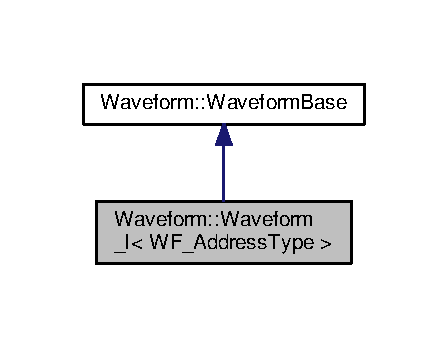
\includegraphics[width=215pt]{class_waveform_1_1_waveform___i__inherit__graph}
\end{center}
\end{figure}


Collaboration diagram for Waveform\+:\+:Waveform\+\_\+I$<$ W\+F\+\_\+\+Address\+Type $>$\+:\nopagebreak
\begin{figure}[H]
\begin{center}
\leavevmode
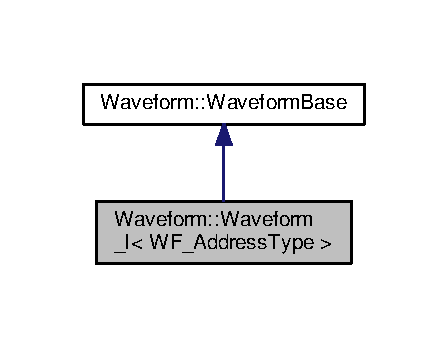
\includegraphics[width=215pt]{class_waveform_1_1_waveform___i__coll__graph}
\end{center}
\end{figure}
\subsection*{Public Types}
\begin{DoxyCompactItemize}
\item 
typedef \hyperlink{class_waveform_1_1_w_f___event}{W\+F\+\_\+\+Event}$<$ W\+F\+\_\+\+R\+E\+C\+V\+\_\+\+M\+S\+G\+\_\+\+E\+VT, \hyperlink{struct_waveform_1_1_w_f___recv_msg_param}{W\+F\+\_\+\+Recv\+Msg\+Param}$<$ W\+F\+\_\+\+Address\+Type $>$ $>$ {\bfseries W\+F\+\_\+\+Rcv\+Message\+Event\+\_\+t}\hypertarget{class_waveform_1_1_waveform___i_ac3fb531925a9157639bf197fee7e8418}{}\label{class_waveform_1_1_waveform___i_ac3fb531925a9157639bf197fee7e8418}

\item 
typedef \hyperlink{class_waveform_1_1_w_f___event}{W\+F\+\_\+\+Event}$<$ W\+F\+\_\+\+D\+A\+T\+A\+\_\+\+N\+T\+Y\+\_\+\+E\+VT, \hyperlink{struct_waveform_1_1_w_f___data_status_param}{W\+F\+\_\+\+Data\+Status\+Param}$<$ W\+F\+\_\+\+Address\+Type $>$ $>$ {\bfseries W\+F\+\_\+\+Data\+Status\+Event\+\_\+t}\hypertarget{class_waveform_1_1_waveform___i_a5efbb2428b3d0dbe51994f70a352a1ba}{}\label{class_waveform_1_1_waveform___i_a5efbb2428b3d0dbe51994f70a352a1ba}

\item 
typedef \hyperlink{class_waveform_1_1_w_f___event}{W\+F\+\_\+\+Event}$<$ W\+F\+\_\+\+L\+I\+N\+K\+\_\+\+E\+S\+T\+\_\+\+E\+VT, \hyperlink{struct_core_1_1_w_f___link_estimation_param}{W\+F\+\_\+\+Link\+Estimation\+Param}$<$ W\+F\+\_\+\+Address\+Type $>$ $>$ {\bfseries W\+F\+\_\+\+Link\+Estimate\+Event\+\_\+t}\hypertarget{class_waveform_1_1_waveform___i_a90a5d0b20f5e152b91d3e9701c9db069}{}\label{class_waveform_1_1_waveform___i_a90a5d0b20f5e152b91d3e9701c9db069}

\end{DoxyCompactItemize}
\subsection*{Public Member Functions}
\begin{DoxyCompactItemize}
\item 
\hyperlink{class_waveform_1_1_waveform___i_a98959d954f80b314ef896d2f857b7e4c}{Waveform\+\_\+I} (Waveform\+Id\+\_\+t \+\_\+w\+Id, \hyperlink{namespace_waveform_a8362d1abeefedecd1142a174faedc096}{W\+F\+\_\+\+TypeE} \+\_\+type, \hyperlink{namespace_waveform_a264307e95d31e27c5a69031fd2615f98}{W\+F\+\_\+\+Estimator\+TypeE} \+\_\+est\+Type, char $\ast$\+\_\+device\+Name)
\begin{DoxyCompactList}\small\item\em Constructor. Creates a waveform object. \end{DoxyCompactList}\item 
virtual void \hyperlink{class_waveform_1_1_waveform___i_ab651687e82a54481718d2ee75e40ec53}{Send\+Data} (\hyperlink{class_waveform_1_1_w_f___message_t}{W\+F\+\_\+\+MessageT}$<$ W\+F\+\_\+\+Address\+Type $>$ \&\+\_\+msg, uint16\+\_\+t \+\_\+payload\+Size, W\+F\+\_\+\+Address\+Type $\ast$\+\_\+dest\+Array, uint16\+\_\+t \+\_\+no\+Of\+Dest, W\+F\+\_\+\+Message\+Id\+\_\+t \+\_\+msg\+Id, bool \+\_\+no\+Ack=false)=0
\begin{DoxyCompactList}\small\item\em Send message indicated by the Message\+Id to a set of neighbors indicated by dest\+Array, with a given payload size. \end{DoxyCompactList}\item 
virtual void \hyperlink{class_waveform_1_1_waveform___i_ac2ddb96d5fb3c8cd410f688acde95389}{Broadcast\+Data} (\hyperlink{class_waveform_1_1_w_f___message_t}{W\+F\+\_\+\+MessageT}$<$ W\+F\+\_\+\+Address\+Type $>$ \&\+\_\+msg, uint16\+\_\+t \+\_\+payload\+Size, W\+F\+\_\+\+Message\+Id\+\_\+t \+\_\+msg\+Id)
\begin{DoxyCompactList}\small\item\em Sends a broadcast on a waveform. Destination received data notification will not be generated If the waveform does not support physical layer broadcasting, the implementation is upto the waveform or the waveform might simply not implement this interface. \end{DoxyCompactList}\item 
virtual void \hyperlink{class_waveform_1_1_waveform___i_a0dc200e92cdff86e55d65ab270c988e6}{Cancel\+Data\+Request} (Request\+Id\+\_\+t \+\_\+r\+Id, W\+F\+\_\+\+Message\+Id\+\_\+t \+\_\+msg\+Id, W\+F\+\_\+\+Address\+Type $\ast$\+\_\+dest\+Array, uint16\+\_\+t \+\_\+no\+Of\+Destinations)=0
\begin{DoxyCompactList}\small\item\em Requests the Cancellation of a data message already sent to the waveform for one or more destinations. \end{DoxyCompactList}\item 
virtual void \hyperlink{class_waveform_1_1_waveform___i_ace837715041bdea1e7857ccd9858e3f2}{Add\+Destination\+Request} (Request\+Id\+\_\+t \+\_\+r\+Id, W\+F\+\_\+\+Message\+Id\+\_\+t \+\_\+msg\+Id, W\+F\+\_\+\+Address\+Type $\ast$\+\_\+dest\+Array, uint16\+\_\+t \+\_\+no\+Of\+Destinations)=0
\begin{DoxyCompactList}\small\item\em Adds one or more destinations to a packet, that has already been sent to the waveform. \hyperlink{namespace_waveform}{Waveform} will send a Control Response Event as reply to this command. \end{DoxyCompactList}\item 
virtual \hyperlink{class_waveform_1_1_waveform___i_a1f0f3d3a86e5b34ca19d84a5425ea7ba}{$\sim$\+Waveform\+\_\+I} ()\hypertarget{class_waveform_1_1_waveform___i_a1f0f3d3a86e5b34ca19d84a5425ea7ba}{}\label{class_waveform_1_1_waveform___i_a1f0f3d3a86e5b34ca19d84a5425ea7ba}

\begin{DoxyCompactList}\small\item\em virtual destructor for interface \end{DoxyCompactList}\end{DoxyCompactItemize}
\subsection*{Protected Attributes}
\begin{DoxyCompactItemize}
\item 
Waveform\+Id\+\_\+t {\bfseries W\+ID}\hypertarget{class_waveform_1_1_waveform___i_af7ee22c008f34e6ba23a8fe00f3db901}{}\label{class_waveform_1_1_waveform___i_af7ee22c008f34e6ba23a8fe00f3db901}

\item 
\hyperlink{namespace_waveform_a8362d1abeefedecd1142a174faedc096}{W\+F\+\_\+\+TypeE} {\bfseries wf\+Type}\hypertarget{class_waveform_1_1_waveform___i_a932ddf78b5aa0eab3b38f3ecddebb00a}{}\label{class_waveform_1_1_waveform___i_a932ddf78b5aa0eab3b38f3ecddebb00a}

\item 
char {\bfseries device\+Name} \mbox{[}32\mbox{]}\hypertarget{class_waveform_1_1_waveform___i_ae1d816e833a5a5941cb8fa3d8567508b}{}\label{class_waveform_1_1_waveform___i_ae1d816e833a5a5941cb8fa3d8567508b}

\item 
\hyperlink{namespace_waveform_a264307e95d31e27c5a69031fd2615f98}{W\+F\+\_\+\+Estimator\+TypeE} {\bfseries est\+Type}\hypertarget{class_waveform_1_1_waveform___i_a08a164eba2b7d5dceb88755dc39acaf4}{}\label{class_waveform_1_1_waveform___i_a08a164eba2b7d5dceb88755dc39acaf4}

\end{DoxyCompactItemize}


\subsection{Detailed Description}
\subsubsection*{template$<$class W\+F\+\_\+\+Address\+Type$>$\\*
class Waveform\+::\+Waveform\+\_\+\+I$<$ W\+F\+\_\+\+Address\+Type $>$}

Defines the generic iteractions for waveforms. 

The interface defines a asynchornous message passing interface for interacting with a waveform running either as part of same process or as seperate process on the same node. When running as two seperate processes, a shim-\/layer will be implementation that will translate the calls between the two processes.

The control flow in general consist of a command/request orginating from the framework to the waveform and the waveform responding to the command/request using a event response. There four types of events that the waveform can send to the framework \+:
\begin{DoxyEnumerate}
\item Response Event (W\+F\+\_\+\+Control\+Response\+Event\+\_\+t)\+: This is called in response to one of the $\ast$\+Request message, with an appropriate response type, response status (sucuss/failure), any additional data and its size
\item Received Message Event (W\+F\+\_\+\+Rcv\+Message\+Event\+\_\+t) \+: This delegate is called whenever a message is received on the waveform, with the message as the parameter
\item Data notification delegate (W\+F\+\_\+\+Data\+Notifier\+Event\+\_\+t)\+: This is called to convey the status of the Send\+Data and Broadcast\+Data calls. The delegates are might be called upto three types for each message, once to acknowledge the message has been received by the waveform, once when it is sent out and once when the message is received at the destination.
\item Link estimation delegate (W\+F\+\_\+\+Link\+Estimates\+Event\+\_\+t)\+: This is called by waveform to provide link estiamtions about neighbors to the framework, if the waveform can provide link estimates. 
\end{DoxyEnumerate}

\subsection{Constructor \& Destructor Documentation}
\index{Waveform\+::\+Waveform\+\_\+I@{Waveform\+::\+Waveform\+\_\+I}!Waveform\+\_\+I@{Waveform\+\_\+I}}
\index{Waveform\+\_\+I@{Waveform\+\_\+I}!Waveform\+::\+Waveform\+\_\+I@{Waveform\+::\+Waveform\+\_\+I}}
\subsubsection[{\texorpdfstring{Waveform\+\_\+\+I(\+Waveform\+Id\+\_\+t \+\_\+w\+Id, W\+F\+\_\+\+Type\+E \+\_\+type, W\+F\+\_\+\+Estimator\+Type\+E \+\_\+est\+Type, char $\ast$\+\_\+device\+Name)}{Waveform_I(WaveformId_t _wId, WF_TypeE _type, WF_EstimatorTypeE _estType, char *_deviceName)}}]{\setlength{\rightskip}{0pt plus 5cm}template$<$class W\+F\+\_\+\+Address\+Type$>$ {\bf Waveform\+::\+Waveform\+\_\+I}$<$ W\+F\+\_\+\+Address\+Type $>$\+::{\bf Waveform\+\_\+I} (
\begin{DoxyParamCaption}
\item[{Waveform\+Id\+\_\+t}]{\+\_\+w\+Id, }
\item[{{\bf W\+F\+\_\+\+TypeE}}]{\+\_\+type, }
\item[{{\bf W\+F\+\_\+\+Estimator\+TypeE}}]{\+\_\+est\+Type, }
\item[{char $\ast$}]{\+\_\+device\+Name}
\end{DoxyParamCaption}
)}\hypertarget{class_waveform_1_1_waveform___i_a98959d954f80b314ef896d2f857b7e4c}{}\label{class_waveform_1_1_waveform___i_a98959d954f80b314ef896d2f857b7e4c}


Constructor. Creates a waveform object. 

{\bfseries  Semantic Behavior\+:} The constructor is expected to create and initialize the waveform object. The constructor is also expected to “connect” to the Framework process. The mechanism of connecting may be platform specific. The data plane of the waveform is expected to be in W\+F\+\_\+\+N\+O\+R\+M\+AL state at the end of this call.

The Waveform\+Id is allocated statically during compile time in the current version of Tuscarora. Other parameters of the constructor are decided by the waveform provider.


\begin{DoxyParams}{Parameters}
{\em \+\_\+w\+Id} & Unique ID of the waveform. The Waveform\+Id is allocated when the Tuscarora is initialized. A waveform writter usually doesnot have to worry about how they are generated. A waveform is expected to store this ID and use it to uniquely identify itself when communicating with the framework. \\
\hline
{\em \+\_\+type} & Type of the waveform. This is one of the types of the waveform the framework supports. \\
\hline
{\em \+\_\+est\+Type} & Type of the estimator provided by the waveform. Indicated weather or not the waveform supports link estimation. \\
\hline
{\em \+\_\+device\+Name} & Name of the device which will be used by the waveform, if device names exist on the platform used to deploy the waveform. \\
\hline
\end{DoxyParams}


\subsection{Member Function Documentation}
\index{Waveform\+::\+Waveform\+\_\+I@{Waveform\+::\+Waveform\+\_\+I}!Add\+Destination\+Request@{Add\+Destination\+Request}}
\index{Add\+Destination\+Request@{Add\+Destination\+Request}!Waveform\+::\+Waveform\+\_\+I@{Waveform\+::\+Waveform\+\_\+I}}
\subsubsection[{\texorpdfstring{Add\+Destination\+Request(\+Request\+Id\+\_\+t \+\_\+r\+Id, W\+F\+\_\+\+Message\+Id\+\_\+t \+\_\+msg\+Id, W\+F\+\_\+\+Address\+Type $\ast$\+\_\+dest\+Array, uint16\+\_\+t \+\_\+no\+Of\+Destinations)=0}{AddDestinationRequest(RequestId_t _rId, WF_MessageId_t _msgId, WF_AddressType *_destArray, uint16_t _noOfDestinations)=0}}]{\setlength{\rightskip}{0pt plus 5cm}template$<$class W\+F\+\_\+\+Address\+Type$>$ virtual void {\bf Waveform\+::\+Waveform\+\_\+I}$<$ W\+F\+\_\+\+Address\+Type $>$\+::Add\+Destination\+Request (
\begin{DoxyParamCaption}
\item[{Request\+Id\+\_\+t}]{\+\_\+r\+Id, }
\item[{W\+F\+\_\+\+Message\+Id\+\_\+t}]{\+\_\+msg\+Id, }
\item[{W\+F\+\_\+\+Address\+Type $\ast$}]{\+\_\+dest\+Array, }
\item[{uint16\+\_\+t}]{\+\_\+no\+Of\+Destinations}
\end{DoxyParamCaption}
)\hspace{0.3cm}{\ttfamily [pure virtual]}}\hypertarget{class_waveform_1_1_waveform___i_ace837715041bdea1e7857ccd9858e3f2}{}\label{class_waveform_1_1_waveform___i_ace837715041bdea1e7857ccd9858e3f2}


Adds one or more destinations to a packet, that has already been sent to the waveform. \hyperlink{namespace_waveform}{Waveform} will send a Control Response Event as reply to this command. 

{\bfseries  Semantic Behavior\+:} \hyperlink{namespace_waveform}{Waveform} should add a destination to the outgoing message if it has not already sent out the message identified by the message ID and send a positive response. If the waveform has already sent out the message to all the destinations and has cleaned its local buffers of the message, it should send a negative response to this request. Once destination has been added to a message, the waveform should communicate the result of the operation using Data Status Response Events as usual.

A response to this request should be generated through the Control Response Event, with the same Request\+ID, that should include a status which will be set to false if the message has been sent out or if the waveform is otherwise unable to add destinations to the message. Otherwise the status should be set to true in the response message.


\begin{DoxyParams}{Parameters}
{\em \+\_\+r\+Id} & Specifies the ID of the request, which the waveform will use in its response message \\
\hline
{\em \+\_\+msg\+Id} & ID of the message that to which the destinations needs to be added \\
\hline
{\em \+\_\+dest\+Array} & New destinations to be added to the message \\
\hline
{\em \+\_\+no\+Of\+Destinations} & Number of destinations in the dest\+Array. If this is 0, the request will be ignored by waveform. \\
\hline
\end{DoxyParams}
\begin{DoxyReturn}{Returns}
void 
\end{DoxyReturn}


Implemented in \hyperlink{class_waveform_1_1_waveform__64b___i_a9b0bcd9f799da0bcb6bb9984679b0e19}{Waveform\+::\+Waveform\+\_\+64b\+\_\+I}.

\index{Waveform\+::\+Waveform\+\_\+I@{Waveform\+::\+Waveform\+\_\+I}!Broadcast\+Data@{Broadcast\+Data}}
\index{Broadcast\+Data@{Broadcast\+Data}!Waveform\+::\+Waveform\+\_\+I@{Waveform\+::\+Waveform\+\_\+I}}
\subsubsection[{\texorpdfstring{Broadcast\+Data(\+W\+F\+\_\+\+Message\+T$<$ W\+F\+\_\+\+Address\+Type $>$ \&\+\_\+msg, uint16\+\_\+t \+\_\+payload\+Size, W\+F\+\_\+\+Message\+Id\+\_\+t \+\_\+msg\+Id)}{BroadcastData(WF_MessageT< WF_AddressType > &_msg, uint16_t _payloadSize, WF_MessageId_t _msgId)}}]{\setlength{\rightskip}{0pt plus 5cm}template$<$class W\+F\+\_\+\+Address\+Type$>$ virtual void {\bf Waveform\+::\+Waveform\+\_\+I}$<$ W\+F\+\_\+\+Address\+Type $>$\+::Broadcast\+Data (
\begin{DoxyParamCaption}
\item[{{\bf W\+F\+\_\+\+MessageT}$<$ W\+F\+\_\+\+Address\+Type $>$ \&}]{\+\_\+msg, }
\item[{uint16\+\_\+t}]{\+\_\+payload\+Size, }
\item[{W\+F\+\_\+\+Message\+Id\+\_\+t}]{\+\_\+msg\+Id}
\end{DoxyParamCaption}
)\hspace{0.3cm}{\ttfamily [inline]}, {\ttfamily [virtual]}}\hypertarget{class_waveform_1_1_waveform___i_ac2ddb96d5fb3c8cd410f688acde95389}{}\label{class_waveform_1_1_waveform___i_ac2ddb96d5fb3c8cd410f688acde95389}


Sends a broadcast on a waveform. Destination received data notification will not be generated If the waveform does not support physical layer broadcasting, the implementation is upto the waveform or the waveform might simply not implement this interface. 

{\bfseries  Semantic Behavior\+:} Broadcast is an optional feature for waveforms. They can choose not to implement it. If implemented, the waveform should set the ‘broadcast\+Support’ field in its Attribute as true whenever it responds to the Attribute\+Request. When the Framework makes a broadcast request, it is expected that the waveform will transmit the message without any specific addressing and without any expectation of destination acknowledgements. The waveform should perform sufficient effort such that neighboring nodes as well as nodes that could be a neighbor might sometimes receive the packet under representative operating conditions.

Efficiency is the key intent of the broadcast method. For example, if a waveform has neighbors across 7 different spectral-\/temporal channels and to reach all of the known neighbors it has to send the same message 7 times, once on each channel, then the nominal implementation would randomly select a channel and send one message on that channel. The randomization ensures that any given neighbor will be reached at least sometimes.

The Message\+Id may be used by the pattern to cancel or replace the payload in future. The waveform is expected to generate 2 notifications through the Data Notification Event, for every message sent to it, the first indicating that the waveform has received the message and the second indicating that it has sent out the message. The waveform can generate a third notification indicating that the destination(s) has received the message if it can support destination acknowledgements.


\begin{DoxyParams}{Parameters}
{\em msg} & Reference to the packet to be broadcasted \\
\hline
{\em payload\+Size} & Size of the payload in the packet. \\
\hline
{\em msg\+Id} & Specifies the id of the framework will use to identify this packet in future calls. \\
\hline
\end{DoxyParams}
\begin{DoxyReturn}{Returns}
void. 
\end{DoxyReturn}


Reimplemented in \hyperlink{class_waveform_1_1_waveform__64b___i_a7ba5150aa1b4e3a123f75dd80ce6ec5b}{Waveform\+::\+Waveform\+\_\+64b\+\_\+I}.

\index{Waveform\+::\+Waveform\+\_\+I@{Waveform\+::\+Waveform\+\_\+I}!Cancel\+Data\+Request@{Cancel\+Data\+Request}}
\index{Cancel\+Data\+Request@{Cancel\+Data\+Request}!Waveform\+::\+Waveform\+\_\+I@{Waveform\+::\+Waveform\+\_\+I}}
\subsubsection[{\texorpdfstring{Cancel\+Data\+Request(\+Request\+Id\+\_\+t \+\_\+r\+Id, W\+F\+\_\+\+Message\+Id\+\_\+t \+\_\+msg\+Id, W\+F\+\_\+\+Address\+Type $\ast$\+\_\+dest\+Array, uint16\+\_\+t \+\_\+no\+Of\+Destinations)=0}{CancelDataRequest(RequestId_t _rId, WF_MessageId_t _msgId, WF_AddressType *_destArray, uint16_t _noOfDestinations)=0}}]{\setlength{\rightskip}{0pt plus 5cm}template$<$class W\+F\+\_\+\+Address\+Type$>$ virtual void {\bf Waveform\+::\+Waveform\+\_\+I}$<$ W\+F\+\_\+\+Address\+Type $>$\+::Cancel\+Data\+Request (
\begin{DoxyParamCaption}
\item[{Request\+Id\+\_\+t}]{\+\_\+r\+Id, }
\item[{W\+F\+\_\+\+Message\+Id\+\_\+t}]{\+\_\+msg\+Id, }
\item[{W\+F\+\_\+\+Address\+Type $\ast$}]{\+\_\+dest\+Array, }
\item[{uint16\+\_\+t}]{\+\_\+no\+Of\+Destinations}
\end{DoxyParamCaption}
)\hspace{0.3cm}{\ttfamily [pure virtual]}}\hypertarget{class_waveform_1_1_waveform___i_a0dc200e92cdff86e55d65ab270c988e6}{}\label{class_waveform_1_1_waveform___i_a0dc200e92cdff86e55d65ab270c988e6}


Requests the Cancellation of a data message already sent to the waveform for one or more destinations. 

{\bfseries  Semantic Behavior\+:} \hyperlink{namespace_waveform}{Waveform} should cancel the transmission of the message, passed in an earlier call to Send\+Data or Broadcast\+Data method with the given message ID, if the message has not been sent out. The message transmission should be cancelled only for the destinations passed as parameters. If the no\+Of\+Destinations parameter is 0, then the entire message should be cancelled. If the message ID is for a Broadcast message the whole message should be cancelled.

A response message should be generated through the Control Response Event, with the same Request\+ID, that should include a status which will be set to false if the message has been sent out or if the waveform is otherwise unable to cancel the transmissions. Otherwise the status should be set to true in the response message.


\begin{DoxyParams}{Parameters}
{\em r\+Id} & Specifies the ID of the request, which the waveform will use to in its response message. \\
\hline
{\em msg\+Id} & ID of the message that needs to be cancelled. \\
\hline
{\em dest\+Array} & Array of destinations to which the packet should be cancelled. \\
\hline
{\em no\+Of\+Destinations} & Number of destinations in the dest\+Array. If the number of destinations is 0, the entire message is cancelled. \\
\hline
\end{DoxyParams}
\begin{DoxyReturn}{Returns}
void 
\end{DoxyReturn}


Implemented in \hyperlink{class_waveform_1_1_waveform__64b___i_a070ad8ff9d1a4a6d66cfaa4bae072752}{Waveform\+::\+Waveform\+\_\+64b\+\_\+I}.

\index{Waveform\+::\+Waveform\+\_\+I@{Waveform\+::\+Waveform\+\_\+I}!Send\+Data@{Send\+Data}}
\index{Send\+Data@{Send\+Data}!Waveform\+::\+Waveform\+\_\+I@{Waveform\+::\+Waveform\+\_\+I}}
\subsubsection[{\texorpdfstring{Send\+Data(\+W\+F\+\_\+\+Message\+T$<$ W\+F\+\_\+\+Address\+Type $>$ \&\+\_\+msg, uint16\+\_\+t \+\_\+payload\+Size, W\+F\+\_\+\+Address\+Type $\ast$\+\_\+dest\+Array, uint16\+\_\+t \+\_\+no\+Of\+Dest, W\+F\+\_\+\+Message\+Id\+\_\+t \+\_\+msg\+Id, bool \+\_\+no\+Ack=false)=0}{SendData(WF_MessageT< WF_AddressType > &_msg, uint16_t _payloadSize, WF_AddressType *_destArray, uint16_t _noOfDest, WF_MessageId_t _msgId, bool _noAck=false)=0}}]{\setlength{\rightskip}{0pt plus 5cm}template$<$class W\+F\+\_\+\+Address\+Type$>$ virtual void {\bf Waveform\+::\+Waveform\+\_\+I}$<$ W\+F\+\_\+\+Address\+Type $>$\+::Send\+Data (
\begin{DoxyParamCaption}
\item[{{\bf W\+F\+\_\+\+MessageT}$<$ W\+F\+\_\+\+Address\+Type $>$ \&}]{\+\_\+msg, }
\item[{uint16\+\_\+t}]{\+\_\+payload\+Size, }
\item[{W\+F\+\_\+\+Address\+Type $\ast$}]{\+\_\+dest\+Array, }
\item[{uint16\+\_\+t}]{\+\_\+no\+Of\+Dest, }
\item[{W\+F\+\_\+\+Message\+Id\+\_\+t}]{\+\_\+msg\+Id, }
\item[{bool}]{\+\_\+no\+Ack = {\ttfamily false}}
\end{DoxyParamCaption}
)\hspace{0.3cm}{\ttfamily [pure virtual]}}\hypertarget{class_waveform_1_1_waveform___i_ab651687e82a54481718d2ee75e40ec53}{}\label{class_waveform_1_1_waveform___i_ab651687e82a54481718d2ee75e40ec53}


Send message indicated by the Message\+Id to a set of neighbors indicated by dest\+Array, with a given payload size. 

{\bfseries  Semantic Behavior\+:} This is the primary method the Framework uses to request that a message be transmitted by the waveform. The first two parameters are self-\/explanatory. The third parameter is an array of one or more neighbors to which the message is to be sent, each of which are identified by the neighbor’s waveform address. The Framework may use the given Message\+Id to cancel or replace the payload in future . The parameter \+\_\+no\+Ack specifies whether a notification is requested when this message has reached its intended destination(s). A true value for this field means the Framework does not need notifications for this message. If data notifications/acknowledgements are not supported by the waveform, this parameter may be ignored.

{\bfseries Data Notifications\+:} It is recommended that Waveforms support acknowledgements from destinations for unicast and multi-\/cast (in local neighborhood) messages. However this is optional. If the waveform choose to implement receiver acks, it should set the ‘dest\+Receive\+Ack\+Support’ field in the Attribute record as true whenever it responds to the Attribute\+Request. If the waveform does not support this feature, then the framework will implement destination acknowledgements by replying to the source node on receiving messages from the waveform. The Message\+Id may be used by the Framework to cancel or replace the payload in future. The waveform is expected to generate at least 2 notifications through the Data Notification Event, for every message sent to it, the first indicating that the waveform has received the message and the second indicating that it has sent out the message. The waveform can generate a third notification indicating that the destination(s) has received the message if it chooses to support destination acknowledgement.

{\bfseries Performance\+:} A request to send to multiple nodes should be fulfilled via a technique that is no less efficient than a sequence of transmissions to each node. The intent is that more advanced waveforms may internally optimize beyond this base performance level, by combining transmissions when possible and not unduly difficult. Any optimizations that\+: 1) are not naturally supported by the hardware and the waveform, 2) require non-\/local information, or 3) consume an order of magnitude more computational resources than required for the core send operation, should not be supported


\begin{DoxyParams}{Parameters}
{\em msg} & Reference to the packet be sent. \\
\hline
{\em payload\+Size} & Size of the payload in the packet. \\
\hline
{\em dest\+Array} & Array of destinations to which the packet should be sent. \\
\hline
{\em no\+Of\+Dest} & Number of destinations in the dest\+Array. \\
\hline
{\em msg\+Id} & Specifies the packet id the framework will use to identify this packet in future calls. \\
\hline
{\em no\+Ack} & Specifies if acks should not be generated. Defaults option generates acks \\
\hline
\end{DoxyParams}
\begin{DoxyReturn}{Returns}
void. 
\end{DoxyReturn}


Implemented in \hyperlink{class_waveform_1_1_waveform__64b___i_acdbf6669aa2e350f9a4b02b06dd4899e}{Waveform\+::\+Waveform\+\_\+64b\+\_\+I}.



The documentation for this class was generated from the following file\+:\begin{DoxyCompactItemize}
\item 
Tuscarora\+F\+W/\+Include/\+Interfaces/\+Waveform/W\+F\+\_\+\+I.\+h\end{DoxyCompactItemize}

